\documentclass[10pt, letterpaper, titlepage]{article} % Set font here.
% Use 'article' for simple documents; use 'report' for larger documents with chapters;
% use 'book' for even larger documents with parts.
\usepackage[utf8]{inputenc}
\usepackage{geometry}
\usepackage{color,graphicx,overpic} 
\usepackage{fancyhdr} % header/footer stuff
\usepackage{amsmath,amsthm,amsfonts,amssymb}
\usepackage{mathtools} % more math stuff
\usepackage{siunitx} % for SI units, ex. $3.5 ~ \si{kg.s^{-2}}$
\usepackage{hyperref} % for hyperlinks
\usepackage{apple_emoji}
\usepackage{multicol}
\usepackage{array}
\usepackage{float}
\usepackage{blindtext}
\usepackage{longtable}
\usepackage{scrextend}
\usepackage[font=small,labelfont=bf]{caption}
\usepackage[framemethod=tikz]{mdframed}
\usepackage{calc}
\usepackage{titlesec}
\usepackage{listings}
\usepackage[normalem]{ulem}

\usepackage{listings}
\usepackage{xcolor}

\DeclareMathOperator{\di}{d\!} % derivative operator symbol, ex. $\int f(x) \di x$
\newcommand{\Eval}[3]{\left.#1\right\rvert_{#2}^{#3}} % evaluation bar (ex. evaluating integral or $\Eval{F(x)}{0}{2}$)
\newcommand*\B{
\includegraphics[height=1.5em,valign=B,raise=-0.2em]{BigB.png}}
\newcommand*\fire{
\includegraphics[height=1.5em,valign=B,raise=-0.2em]{Fire.png}}

\definecolor{comment}{RGB}{140, 140, 140}
\definecolor{text}{RGB}{204, 204, 204}
\definecolor{string}{rgb}{0.58,0,0}
\definecolor{backcolour}{RGB}{27, 30, 39}
\definecolor{variable}{RGB}{244, 63, 78}

\lstdefinestyle{mystyle}{
    backgroundcolor=\color{backcolour},   
    commentstyle=\color{comment},
    keywordstyle=\color{variable},
    numberstyle=\tiny\color{text},
    stringstyle=\color{string},
    basicstyle=\ttfamily\footnotesize\color{text},
    breakatwhitespace=false,         
    breaklines=true,                 
    captionpos=b,                    
    keepspaces=true,                 
    numbers=left,                    
    numbersep=-10pt,                  
    showspaces=false,                
    showstringspaces=false,
    showtabs=false,                  
    tabsize=4
}

\lstdefinelanguage
   [x64]{Assembler}     % add a "x64" dialect of Assembler
   {morekeywords={	
   }} % etc.
   
\lstdefinelanguage[Motorola68k]{Assembler}{%
	morekeywords={	a0, a1, a2, a3, a4, a5, a6, a7, %
   					d0, d1, d2, d3, d4, d5, d6, d7, %
				   	ABCD,ADD,%
					ADDA,ADDI,ADDQ,ADDX,AND,ANDI,ASL,ASR,BCC,BLS,BCS,BLT,BEQ,BMI,BF,BNE,%
					BGE,BPL,BGT,BT,BHI,BVC,BLE,BVS,BCHG,BCLR,BRA,BSET,BSR,BTST,CHK,CLR,%
					CMP,CMPA,CMPI,CMPM,DBCC,DBLS,DBCS,DBLT,DBEQ,DBMI,DBF,DBNE,DBGE,DBPL,%
					DBGT,DBT,DBHI,DBVC,DBLE,DBVS,DIVS,DIVU,EOR,EORI,EXG,EXT,ILLEGAL,JMP,%
					JSR,LEA,LINK,LSL,LSR,MOVE,MOVEA,MOVEM,MOVEP,MOVEQ,MULS,MULU,NBCD,NEG,%
					NEGX,NOP,NOT,OR,ORI,PEA,RESET,ROL,ROR,ROXL,ROXR,RTE,RTR,RTS,SBCD,%
					SCC,SLS,SCS,SLT,SEQ,SMI,SF,SNE,SGE,SPL,SGT,ST,SHI,SVC,SLE,SVS,STOP,%
					SUB,SUBA,SUBI,SUBQ,SUBX,SWAP,TAS,TRAP,TRAPV,TST,UNLK},%
					sensitive=false,%
					morecomment=[l]*,%
					morecomment=[l] }[keywords,comments,strings]

\lstset{language=[Motorola68k]Assembler}
\lstset{style=mystyle}

\definecolor{mycolor}{rgb}{0, 0, 0}
  

\geometry{top=2.7cm,left=1.8cm,right=1.8cm,bottom=2.7cm}
\setlength{\headheight}{17pt}
\renewcommand{\baselinestretch}{1.5} 
\setlength{\parskip}{0.3cm}
\setlength{\parindent}{0.6cm}
\titlespacing\section{0pt}{12pt plus 4pt minus 2pt}{0pt plus 2pt minus 2pt}

\newcommand{\barrows}{\textcolor{blue}{\Longrightarrow}\quad}
\newcommand{\barrow}{\quad\textcolor{blue}{\Longrightarrow}\quad}  
\newcommand{\sumi}[1][1]{ \sum_{n={#1}}^{\infty} }
\newcommand{\limi}[1][n]{ \lim_{{#1}\to\infty} }

\title{\textbf{\Huge{
\begin{center}
Introduction to\\ Subroutines \\ 😂😂😂 \\
\end{center}
}}}
\author{\B enjamin Kong | 1573684\\Lora Ma ||||| 1570935\\ \\ECE 212 Lab Section H11}

\pagestyle{fancy}
\fancyhf{}
\rhead{\B enjamin Kong \& Lora Ma}
\lhead{\textit{Introduction to Subroutines} 😂😂😂}
\rfoot{Page \thepage}

\begin{document} 
\pagenumbering{gobble} 
\maketitle 
\thispagestyle{empty}
\tableofcontents 
\newpage
\pagenumbering{arabic}

\begin{multicols*}{2}


\section{Introduction}
In any particular program, we often need to perform various sub-tasks many times. 
For example, we may need to sort numbers in an integer array. 
We could write the block of instructions that performs this sub-task over and over again as we need to, but this would be tedious and a waste of memory space. 
Therefore, we code these blocks of repeated instructions somewhere in memory and any time we need to use this block of instructions, we simply tell the program to branch to the location of the block of instructions. 
These blocks of instructions (or sub-tasks) are called \textit{subroutines}. 
The instruction that branches to the subroutine is called a \textit{call} instruction. 
Furthermore, the calling program is called the \textit{caller} and the subroutine itself is called the \textit{callee}. 
Once we reach the last instruction in a subroutine (called the \textit{return} instruction), the subroutine returns to the program that called it. 

In this lab, our objective was to gain experience using subroutines by writing subroutines for a statistics program. 
In specific, we wanted to gain experience
\begin{enumerate}
\item using the STACK (Push and Pop),
\item dividing up existing code into subroutines,
\item calling subroutines/functions, and
\item using basic parameter passing techniques.
\end{enumerate}
The lab was broken up into three parts. 
For part A of the lab, we created a program that prompts the user to enter numbers using the keyboard. 
We also checked that the input met certain restrictions, namely
\begin{itemize}
\item the number of entries must be between 3 and 15,
\item the divisor must be between 2 and 5, and
\item the values entered must be positive.
\end{itemize}

For part B of the lab, we created a subroutine that, based on the input, finds the min, max, mean, and how many numbers were divisible by the divisor and what those numbers were.

For part C of the lab, we created a subroutine that displayed the results from part B on the MTTTY. 
Furthermore, we made the subroutine re-display all the numbers that the user input at the beginning. 

\section{Design}
The UML diagrams and assembler code for each part are in the appendix.

\subsection{Part A}
For part A of the lab, our goal was to create a welcome screen that prompts the user for input and awaits input. 
Upon receiving input, we checked if the input is valid via the following conditions:
\begin{itemize}
\item the number of entries must be between 3 and 15,
\item the divisor must be between 2 and 5, and
\item the values entered must be positive.
\end{itemize}

To prompt the user for input, we used iprintf to output strings stored at the end of the assembler code. 
To use iprintf, we stored the addresses of the string we wanted to output on the stack before entering the subroutine. 
At the end of the subroutine, we popped the element off the stack. 
Further, at the end of each subroutine that prompts the user for input, we used getstring, which stores valid numbers in register \%D0. 
If the input was invalid, we used iprintf to output an error message, prompting the user to re-enter valid input.

\subsection{Part B}
For part B of the lab, we took the input from the user and calculated some statistics from the lab. 
These statistics were the min, max, mean, the number of numbers divisible by the divisor, and the numbers divisible by the divisor themselves. 

In order to calculate these statistics, we iterated through each element the user input. 
To find the min and max, we compared it to the currently stored min and max and updated those values accordingly if the element was found to be the smaller than the currently stored min or if the element was found to be larger than the currently stored max. 
We also checked if the element was divisible by the divisor. 
Lastly, we added the element to a counter such that we could calculate the mean at the end. 
We stored the min, max, and mean at addresses 0x43100008, 0x43100004, and 0x43100000 respectively. 
We also pushed the number of entries divisible by the divisor to the stack at the end of the subroutine. 

\subsection{Part C}
For part C of the lab, our goal was to display the calculated values from part B: the min, max, mean, the number of numbers divisible by the divisor, and the numbers divisible by the divisor themselves. 

In order to display information, we used the iprintf subroutine and defined our strings at the end of the program. To access each item to print, we accessed their location in memory and printed them to the MTTTY console accordingly.

\section{Testing}
Due to the shutdown of the university, we were unable to test our code in-person. 
However, we have outlined how we would have tested our code below for each section.

\subsection{Part A}
For part A, we would have checked that our program outputs the required messages as given in the lab manual. 
These messages would have to be output to the MTTTY in the correct order and at the correct times when user input is needed or input. 
Further, we would have checked that our program outputs the error message if an invalid number was input.

\subsection{Part B}
For part B, we would have checked that our program finds the correct min, max, mean, and the numbers that are divisible by the divisor. 
These values would be based on the input from part A. 
To check if our program calculated these values correctly, we would have looked at the memory location at which the results were stored and compare them manually calculated results.

\subsection{Part C}
For part C, we would have checked that the MTTTY was displaying the correct output and that the output was in the correct order and format (as described in the lab manual). 

\section{Questions}
\begin{enumerate}
\item \textit{Is it always necessary to implement either callee or caller preservation of registers when calling a subroutine? Why?}

It is always necessary. 
A subroutine may be running in several different parts of the program and the data and address registers being used by the subroutine could be overwritten. 
If the program was using these data or address registers to store information and this information gets overwritten by the subroutine, it could cause errors or cause unexpected behavior.

\item \textit{Is it always necessary to clean up the stack? Why?}

It is always necessary. 
Let's say the subroutine only restores old register values, but doesn't clean up the stack. 
If the program that called the subroutine relies on information from the stack, the offset of the stack pointer may not be correct and the program would not be accessing the correct information. 

\item \textit{If a proper check for the getstring function was not provided and you have access to the buffer, how would you check to see if a valid \# was entered? A detailed description is sufficient. You do not need to implement this in your code.}

In order to check if a valid \# was input, our program would iterate through each element in the buffer. 
For each element, we would check to see if the character was between `0' and `9'; this could be accomplished using branches. 
If the input was not valid, a message could be output signifying an invalid entry and a prompt could be displayed to have the user re-enter a valid input. 
\end{enumerate}

\section{Conclusion}
The objective of this lab was to explore the use of subroutines for creating a statistics program. 
We were unable to test our code in-person; however, we are confident that our code functions correctly. 
At the end of the day, even if there are a few small bugs in our code, we successfully expanded our knowledge of subroutines substantially.

In part A of the lab, we wrote a program that welcomed the user and promoted the user to enter numbers using the keyboard (using the MTTTY terminal). 
If we had been able to test our code in-person, we would have checked that the inputs met certain requirements as mentioned in the introduction and design section. 

In part B of the lab, we wrote a program that, based on the previous input, found the min, max, mean, how many numbers were divisible by the divisor, and what those numbers were. 
In part C of the lab, we finished our program and made it so that it displayed the values we found in part B. 
We believe that these two parts of the lab were completed successfully as well. 

\end{multicols*}

\newpage

\section{Appendix}

\subsection{Part A UML Diagram}
\begin{figure}[H]
   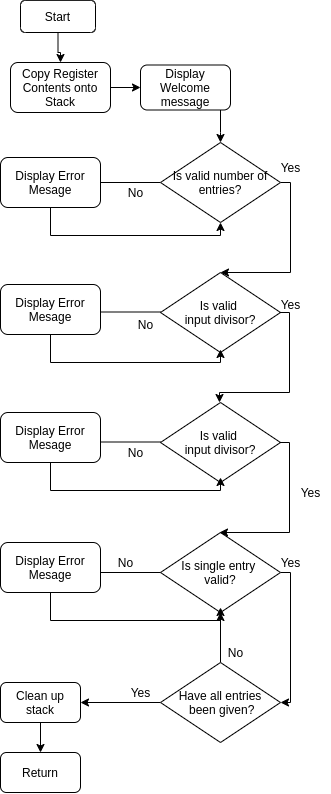
\includegraphics[width=0.4\textwidth]{UMLA.png}
   \centering  
   \caption{UML diagram for part A.} 
   \label{figure:1}
\end{figure}

\subsection{Part B UML Diagram}
\begin{figure}[H]
   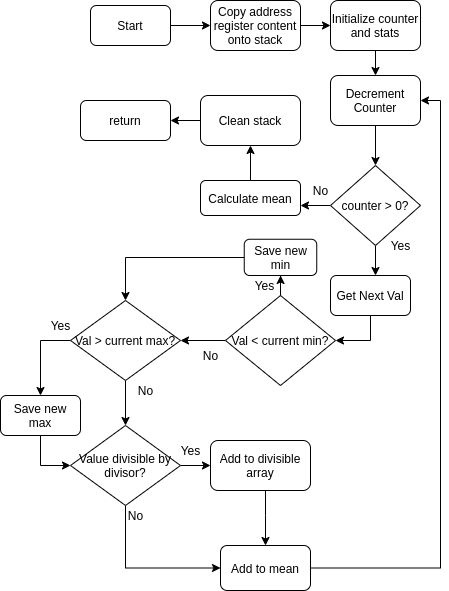
\includegraphics[width=0.6\textwidth]{UMLB.png}
   \centering  
   \caption{UML diagram for part B.} 
   \label{figure:2}
\end{figure}

\subsection{Part C UML Diagram}
\begin{figure}[H]
   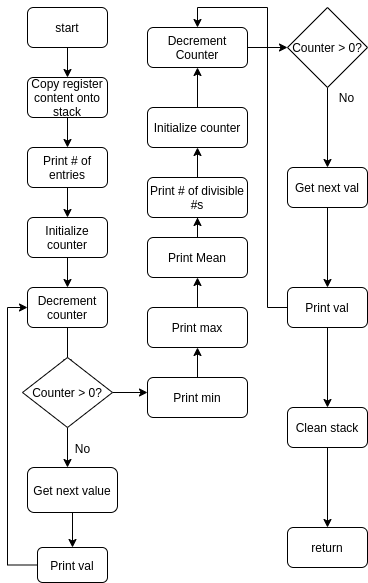
\includegraphics[width=0.4\textwidth]{UMLC.png}
   \centering  
   \caption{UML diagram for part C.} 
   \label{figure:3}
\end{figure}

\newpage

\subsection{Part A Assembler Code}
\begin{lstlisting}
	WelcomePrompt:
	/*Write your program here******************************************/
	
	/* Backup registers */
	lea -40(%sp), %sp
	movem.l %d2-%d7/%a2-%a5, (%sp)
	
	/* Print Welcome message */
	Welcomemsg:
	  pea Welcome /*Push string to stack*/
	  jsr iprintf /*Display string */
	  adda.l #4, %sp /*Pop string location from stack*/
	  jsr cr /*New Line*/
	
	Entries:
	  pea EntriesPrompt /*Push string to stack*/
	  jsr iprintf /*Display string */
	  adda.l #4, %sp /*Pop string location from stack*/
	  jsr cr /*New Line*/
	  jsr getstring /*Get user input*/
	  bra CheckEntry /*Check entry*/
	
	CheckEntry:
	  cmpi.l #15, %d0 /* Compare d0 with 15 */
	  bgt InvalidEntry /* If greater than 15, go to InvalidEntry */
	  cmpi.l #3, %d0 /* Compare d0 with 3 */
	  blt InvalidEntry /* if less than 3, go to InvalidEntry */
	  cmpi.l #0,  %d0 /* compare d0 with 0 */
	  beq exit /*If equal to zero, exit */
	  move.l %d0, 48(%sp) /* Move number of entries onto stack */
	  move.l %d0, %d2 /* Create counter from input */
	
	InvalidEntry:
	  pea Invalid /*Push string to stack*/
	  jsr iprintf /*Display string */
	  adda.l #4, %sp /*Pop string location from stack*/
	  jsr cr /*New Line*/
	  jsr getstring /*Get user input*/
	
	/* Ask for divisor */
	Divisormsg:
	  pea  DivisorPrompt /*Push string to stack*/
	  jsr iprintf /*Display string */
	  adda.l #4, %sp /*Pop string location from stack*/
	  jsr cr /*New Line*/
	  jsr getstring /*Get user input*/
	  bra CheckDiv
	
	InvalidDiv:
	  pea Invalid /*Push string to stack*/
	  jsr iprintf /*Display string */
	  adda.l #4, %sp /*Pop string location from stack*/
	  jsr cr /*New Line*/
	  jsr getstring /*Get user input*/
	
	CheckDiv:
	  cmpi.l #2, %d0 /*Compare d0 with 2*/
	  blt InvalidDiv /*if less than, go to InvalidDiv*/
	  cmpi.l #5, %d0 /*Compare d0 with 5*/
	  bgt InvalidDiv /*If greater than 5, go to InvalidDiv*/
	  move.l %d0, 44(%sp) /* Move divisor number onto stack */
	
	movea.l     #0x43000000, %a2 /* Pointer to array storing data */
	Numbermsg:
	  pea NumberPrompt /*Push string to stack*/
	  jsr iprintf /*Display string */
	  adda.l #4, %sp /*Pop string location from stack*/
	  jsr cr /*New Line*/
	  jsr getstring /*Get user input*/
	  bra CheckNum /* go to CheckNum */
	
	InvalidNum:
	  pea Invalid /*Push string to stack*/
	  jsr iprintf /*Display string */
	  adda.l #4, %sp /*Pop string location from stack*/
	  jsr cr /*New Line*/
	  jsr getstring /*Get user input*/
	
	CheckNum:
	  cmpi.l #0, %d0 /* Check if negative number entered */
	  blt InvalidNum /*Invalid if negative*/
	  move.l %d0, (%a2)+ /*If positive, move to array, increment pointer*/
	  sub.l #1, %d2 /*Decrement counter*/
	  cmpi.l #1, %d2
	  beq LastNummsg /*If last number, go to LastNummsg*/
	  bra Numbermsg /*Otherwise, check next number*/
	
	LastNummsg:
	  pea LastNumPrompt /*Push string to stack*/
	  jsr iprintf /*Display string */
	  adda.l #4, %sp /*Pop string location from stack*/
	  jsr cr /*New Line*/
	  jsr getstring /*Get user input*/
	  bra LastCheck /*Go to LastCheck*/
	
	InvalidLast:
	  pea Invalid /*Push string to stack*/
	  jsr iprintf /*Display string */
	  adda.l #4, %sp /*Pop string location from stack*/
	  jsr cr /*New Line*/
	  jsr getstring /*Get user input*/
	
	LastCheck:
	  cmpi.l #0, %d0
	  blt InvalidLast
	  move.l %d0, (%a2)
	
	exit:
	  /* Restore registers */
	  movem.l %d2-%d7/%a2-%a5, (%sp)
	  lea 40(%sp),%sp
	
	rts
	
	/*End of Subroutine ***********************************************s***/
	.data
	/*All Strings placed here **************************************************/
	
	Welcome:
	.string "Welcome to Wing's Stats Program"
	
	EntriesPrompt:
	.string "Please enter the number (3min-15max) of entries followed by 'enter'"
	
	DivisorPrompt:
	.string "Please enter the divisor (2min-5max) followed by 'enter'"
	
	NumberPrompt:
	.string "Please enter a number (positive only)"
	
	LastNumPrompt:
	.string "Please enter the last number (positive only)"
	
	Invalid:
	.string "Invalid entry, please enter a proper value."
	
	/*End of Strings **************************************************/
\end{lstlisting}

\newpage

\subsection{Part B Assembler Code}
\begin{lstlisting}
	Stats:
	/*Write your program here******************************************/
	
	/* Backup registers */
	lea -40(%sp),%sp
	movem.l %d2-%d7/%a2-%a5, (%sp)
	
	FindMin:
	  move.l (%a2)+, %d2
	  move.l 48(%sp), %d4 /*Initialize counter*/
	
	LoopMin:
	  sub.l #1, %d4 /* Decrement counter */
	  move.l (%a2)+, %d3 /* Load Next number to test */
	  cmp.l #0, %d4 /* Check if counter done */
	  ble FindMaxVal /* If counter done, go to FindMaxVal */
	  cmp.l %d3, %d2 /* Compare stored and new number */
	  blt LoopMin /* If stored is smaller, repeat checks */
	  move.l %d3, %d2 /* If stored is larger, save new number */
	  bra LoopMin /* Repeat loop */
	
	FindMaxVal:
	  move.l %d2, (%a3)+ /* Save min number */
	  movea.l #0x43000000, %a2 /* Reinitialize counter to data array */
	  move.l (%a2)+, %d2 /* Load First number */
	  move.l 48(%sp), %d4 /* Reload Counter */
	
	LoopMax:
	  sub.l #1, %d4 /* Decrement counter */
	  move.l (%a2)+, %d3 /* Load Next number to test */
	  cmp.l #0, %d4 /* Check if counter done */
	  ble FindMeanVal /* If counter done, go to FindMaxVal */
	  cmp.l %d3, %d2 /* Compare stored and new number */
	  bgt LoopMax /* If stored is larger, repeat checks */
	  move.l %d3, %d2 /* If stored is smaller, save new number */
	  bra LoopMax /* Repeat loop */
	
	FindMeanVal:
	  move.l %d2, (%a3)+ /* Save max number */
	  movea.l #0x43000000, %a2 /* Reinitialize counter to data array */
	  move.l 48(%sp), %d3 /* Reload Counter */
	  clr.l %d2 /* Clear D5 to use as cum sum */
	
	LoopMean:
	  add.l (%a2)+, %d2 /*Add num at address register to d2 and increment a2*/
	  sub.l #1, %d3 /*Subtract o1 from d3*/
	  bne LoopMean /*If not equal to zero, go to LoopMean*/
	  divu.l 48(%sp), %d2 /*Divide total sum by amount of integers*/
	  move.l %d2, (%a3)+ /*Move mean to output array*/
	
	move.l 48(%sp), %d3 /*Reload Counter*/
	movea.l #0x43000000, %a2 /*Reinitialize counter to data array*/
	move.l #4, %d5 /*Move #4 to d5*/
	clr.l %d6 /*Divisor counter*/
	
	FindDivisible:
	  move.l (%a2)+, %d2 /*Move data at address a2 to d2 and increment a2*/
	  move.l %d2, %d4 /*Move data at d2 to d4*/
	  move.l 44(%sp), %d7 /*Move stack pointer*/
	  divu.w %d7, %d4 /*lower word contains quotient - higher word has remainder*/
	
	Remainder:
	  and.l #0xFFFF0000, %d4
	  cmp.l	#0, %d4 /*Compare #0 with d4*/
	  bne	NotDivisible /*If not equal, go to NotDivisible*/
	  move.l %d2,(%a3)+ /*Move value at d2 to address a3 and increment*/
	  add.l #1, %d6		/*Increment divisor counter*/
	  sub.l #1,%d3 /*Subtract #1 from d3*/
	  bne FindDivisible /*if not equal to zero, go to FindDivisible*/
	  bra exit /*else, exit*/
	
	NotDivisible:
	  sub.l #1, %d3 /*Subtract 1 from d3*/
	  bne FindDivisible /*If not equal to zero, go to FindDivisible*/
	
	exit:
	  move.l %d6, 52(%sp)
	
	
	movem.l (%sp), %d2-%d7/%a2-%a5
	lea 40(%sp), %sp
	rts
	
	/*End of Subroutine **************************************************/
	.data
\end{lstlisting}

\newpage

\subsection{Part C Assembler Code}
\begin{lstlisting}
	Display:
	/*Write your program here******************************************/
	lea -40(%sp), %sp
	movem.l %d2-%d7/%a2-%a5, (%sp)
	
	pea NumPrompt /* Push location of string to stack */
	jsr iprintf /* Print out string */
	adda.l #4, %sp /* Clean up stack */
	
	move.l 48(%sp), %d2 /* Load number */
	move.l %d2, -(%sp) /* Store to stack */
	jsr value /* Print number */
	adda.l #4, %sp /* Clean up stack */
	jsr cr /* Print newline */
	clr.l %d3 /* Prepare counter */
	
	Loop: /* Counter print loop *?
	  move.l (%a2, %d3*4), -(%sp) /* Load number to stack, using counter as index */
	  jsr value /* Print number */
	  jsr cr /* Print newline */
	  adda.l #4, %sp /* Remove number from stack */
	  add.l #1, %d3 /* Increment counter */
	  cmp.l %d2, %d3 /* Check if done */
	  blt Loop /* repeat if not */
	
	pea MinPrompt /* Push string to stack */
	jsr iprintf /* Print out string */
	adda.l #4, %sp /* pop stack */
	move.l (%a3)+, -(%sp) /* Load smallest number to stack */
	jsr value /* Print out number to stack */
	adda.l #4, %sp /* Pop stack */
	jsr cr /* Print newline */
	
	pea MaxPrompt /* Push string to stack */
	jsr iprintf /* Print out string */
	adda.l #4, %sp /* pop stack */
	move.l (%a3)+, -(%sp) /* Load largest number to stack */
	jsr value /* Print out number to stack */
	adda.l #4, %sp /* Pop stack */
	jsr cr /* Print newline */
	
	pea MeanPrompt /* Push string to stack */
	jsr iprintf /* Print out string */
	adda.l #4, %sp /* pop stack */
	move.l (%a3), -(%sp) /* Load average number to stack */
	jsr value /* Print out number to stack */
	adda.l #4, %sp /* Pop stack */
	jsr cr /* Print newline */
	
	pea Divisible1 /* Push string to stack */
	jsr iprintf /* Print out string */
	adda.l #4, %sp /* pop stack */
	move.l 52(%sp), %d2 /* Load number to register */
	move.l %d2, -(%sp) /* Push number to stack */
	jsr value /* Print out number to stack */
	adda.l #4, %sp /* pop stack */
	
	pea Divisible2 /* Push string to stack */
	jsr iprintf /* Print out string */
	adda.l #4, %sp /* pop stack */
	move.l 44(%sp), %d2 /* Load number to register */
	move.l %d2, -(%sp) /* Push number to stack */
	jsr value /* Print out number to stack */
	adda.l #4, %sp /* pop stack */
	
	jsr cr /* Print newline */
	
	pea EndText /* Push end text to stack */
	jsr iprintf /* Print text */
	adda.l #4, %sp /* Pop stack */
	
	jsr cr /* Print newline */
	
	movem.l (%sp), %d2-%d7/%a2-%a5 /* Restore registers */
	lea 40(%sp), %sp /* Reset stack pointer */
	
	rts
	
	/*End of Subroutine **************************************************/
	.data
	/*All Strings placed here **************************************************/
	NumEntriesText:
	.string "The number of entries was "
	
	MinPrompt:
	.string "Min Number = "
	
	MaxPrompt:
	.string "Max Number = "
	
	MeanPrompt:
	.string "Mean Number = "
	
	Divisible1:
	.string "There are "
	
	Divisible2:
	.string " number(s) divisble by "
	
	EndText:
	.string "Program ended"
	
	/*End of Strings **************************************************/
\end{lstlisting}

\end{document}
